\documentclass[a4paper, 11pt]{article}
\usepackage{preamble}
% \usepackage{fullpage}
\usepackage[paper=a4paper,margin=1.5in, includeheadfoot, footskip=30pt]{geometry}
\usepackage{dsfont}
\usepackage{algorithm}
\usepackage{algorithmic}
\usepackage{paralist}
\usepackage{csvsimple}
\usepackage{longtable}
\usepackage{booktabs}
\usepackage{tikz}
\usepackage{afterpage}
\usepackage{multicol}
\usepackage{cleveref}
\usepackage[toc]{appendix}

\hypersetup{
    colorlinks = false,
    linkbordercolor = 1 1 0,
}


\sisetup{range-phrase=-}
\DeclareSIUnit{\au}{a.u.}

\crefformat{footnote}{#2\footnotemark[#1]#3}

\newcommand{\drawfrom}{\overset{\mathrm{d}}{=}}
\newcommand{\setfrom}{\overset{\mathrm{d}}{\leftarrow}}


\title{ \small
University of Oslo\\
FYS4411\\
Computational physics II: Quantum mechanical systems\\
\huge Project 2: The Restricted Boltzmannn Machine Applied to the Quantum Many Body Problem}
\author{\textsc{Bendik Samseth}}
\date{\today}
\begin{document}
\maketitle

\begin{abstract}
    Abstract here, please.
    All material referenced in this report is available at
    \url{https://github.com/bsamseth/FYS4411}.
\end{abstract}


\pagebreak
\newgeometry{margin=0.9in}
\tableofcontents

\begin{multicols}{2}    

    \section{Introduction} 

    A physicist faced with a quantum many body system is quickly forced to
    abandon any hope of solving the Schrödinger equation (or one of its even worse
    relativistic siblings) exactly. Instead he must resort to one of two general
    workarounds: 1) make simplifying assumptions until the equation is solvable,
    or 2) make an educated guess for the solution. In either case, the desired
    quantity which solving the Schrödinger equation would yield is the quantum
    mechanical wavefunction. If we want to stay away from potentially faulty, or
    limiting assumptions, we must therefore somehow produce a guess for this
    wavefunction, without actually solving the equation.

    The last project utilized the Variational Monte Carlo (VMC) approach, in which a
    specific, parametrized form is assumed for the wavefunction, with the
    subsequent optimization of the parameters.

    The main limitation of VMC is that a specific form for the wavefunction is
    assumed. If this form contains the true optimum that works fine, but if not
    we are inherently limited in how accurate the final results can be.

    Aiming to be overcome this issue, we may observe that the task at hand falls
    into the general field of function approximation. We wish to approximate the
    function that takes as input the configuration of the system, and outputs a
    probability amplitude for the given state. Function approximation is a task
    which lends itself to techniques from machine learning (ML). 

    In this project we will attempt to represent the wavefunction with a
    specific type of ML-model, the Restricted Boltzmann Machine (RBM). The use
    of RBMs for such applications was presented recently by
    \textcite{Carleo602}, with encouraging results. We shall therefore attempt
    to apply the same techniques to a different type of system, namely that of
    two interacting quantum particles confined in a harmonic oscillator trap.

    The choice of using the RBM as our model is somewhat arbitrary, and other
    model architectures could also be of interest. The general ML-approach which
    we employ, regardless of the specifics of the underlying model, is as follows:

    \begin{enumerate}
        \item Define the model to be trained.
        \item Formulate the objective, or \emph{loss function}.
        \item Using some optimization scheme, optimize the model wrt. to the
            loss function.
    \end{enumerate}


    \section{Theory}

    \subsection{The System}

    We consider a system of electrons confined in a pure two-dimensional
    isotropic harmonic oscillator potential, with an idealized total Hamiltonian
    given by:

    \begin{align}
        \begin{split}
            \hat H &= \sum_{i=1}^P\qty(-\frac{1}{2}\laplacian_i + V_{ext}(\vec r_i)) +
            \sum_{i < j} V_{int}(\vec r_i, \vec r_j)\\
            &= \sum_{i=1}^P\qty(-\frac{1}{2}\laplacian_i + \frac{1}{2}\omega^2
            r_i^2) + \sum_{i < j} \frac{1}{r_{ij}},
        \end{split}\label{eq:H-def}
    \end{align}
    where natural units ($\hbar=c=m_e=1$) are used with energies in
    atomic units (a.u.), $P$ denotes the number of particles in the system, and
    $\omega$ is the oscillator frequency of the trap. Further, $\vec r_i$
    denotes the position vector of particle $i$, with $r_i \equiv \norm{\vec r}$ and
    $r_{ij}\equiv \norm{\vec r_i - \vec r_j}$ defined for notational brevity.

    In this project we limit ourselves to the case of $N=2$ interacting
    electrons in a trap with a frequency such that $\hbar \omega = 1$. We do
    this because for this case we have exact, analytical solutions for the
    ground state energy. With the interaction term included, the ground state
    energy is $E_0 = \SI{3}{\au}$~\cite{Taut1993}. This limitation is purely one
    of convenience, as having exact benchmarks makes for better verification of
    results. The methods discussed in the project should extend to other
    systems.

    \subsection{Simple Non-Interacting Case}
    If we omit the interacting terms in \autoref{eq:H-def} we have
    the standard harmonic oscillator Hamiltonian:
    \begin{align}
        \hat H_0 &= \sum_{i=1}^P\qty(-\frac{1}{2}\laplacian_i +
        \frac{1}{2}\omega^2 r_i^2).
    \end{align}
    This Hamiltonian lends it self to analytical solutions, and the stationary
    states are:
    \begin{align}
        \phi_{n_x, n_y}(x, y) &= A H_{n_x}(\sqrt\omega x)H_{n_y}(\sqrt\omega y)
        e^{-\frac{\omega}{2}\qty(x^2 + y^2)},
    \end{align} 
    for quantum numbers $n_x, n_y = 0, 1,\dots$, and the Hermite polynomials
    $H_n$. The ground state, $n_x=n_y=0$ is simply
    \begin{align}
        \phi_{00}(x,y) =
        \sqrt{\frac{\omega}{\pi}}e^{-\frac{\omega}{2}\qty(x^2+y^2)}.
    \end{align}
    Using this wavefunction we can calculate the ground state
    energy\footnote{\label{fnt:sympy}See \texttt{projects/python/Sympy.ipynb} in the Github
    repository for an explicit calculation of the ground state energy},
    \begin{align}
        \epsilon_{00} = \frac{\expval{\hat H_0}{\phi_{00}}}{\braket{\phi_{00}}}
        = \omega = \SI{1}{\au}
    \end{align}

    The ground state wavefunction for the (unperturbed) two-electron case is simply the
    product of the one-electron wavefunctions,
    \begin{align}
        \begin{split}
            \Phi(\vec r_1, \vec r_2) &= \phi_{00}(\vec r_1)\phi_{00}(\vec r_2)\\
            &= \frac{\omega}{\pi} e^{-\frac{\omega}{2}\qty(r_1^2+r_2^2)}.
        \end{split}\label{eq:Phi-non-inter}
    \end{align}

    The ground state energy can once again be evaluated
    analytically\cref{fnt:sympy} and yields
    \begin{align}
        E_0 = \frac{\expval{\hat H_0}{\Phi}}{\braket{\Phi}}
        = 2\omega =\SI{2}{\au}
    \end{align}
    This result is not surprising, as adding one more particle, without any
    interactions, should simply double the energy. Another way to look at it is
    that the simple harmonic oscillator solution gives $\flatfrac{\omega}{2}$
    per degree of freedom, so adding another two yields and extra $\omega$.


    When the two particles are electrons, we may say something about their total
    spin. As electrons are fermions, their total wavefunction must be
    anti-symmetric upon interchanging the labels $1$ and $2$.
    \autoref{eq:Phi-non-inter} is obviously symmetric, and so the
    spin-wavefunction must necessarily be anti-symmetric. For the combination of
    two spin-1/2 particles, there is only one candidate, namely the spin-0
    singlet:

    \begin{align}
        \chi_0 = \frac{1}{\sqrt 2}\qty(\ket{\uparrow\downarrow} -
        \ket{\downarrow\uparrow}).
    \end{align}

    \section{Representing the Wavefunction with an RBM}

    Our machine learning model of choice is the Restricted Boltzmann Machine. It
    consists of of two densely interconnected layers, the \emph{visible} layer
    and the \emph{hidden} layer. It is called restricted because we only
    allow connections between nodes in different layers - no visible-to-visible or
    hidden-to-hidden connections are included.

    The RBM is a generative model, meaning it learns a probability distribution
    for its inputs. This means that a trained RBM can produce outputs which
    when viewed as a distribution, would be similar to the distribution of the
    inputs. For our case, this means learning the probability distribution for
    the space configurations of the electrons in our system. We may interpret
    this distribution as the wavefunction, as the wavefunction serves this same
    purpose.

    In this case we do not have a training set of positions for any of the
    systems under consideration. This means that the most desired training
    regime, \emph{supervised training}, is not relevant for our problem. Instead
    we shall use \emph{reinforcement training}, were updates of the model are
    based on the variational principle: The true ground state wavefunction is
    the wavefunction for which the lowest ground state energy is obtained. We
    can treat the energy that a certain wavefunction (model configuration)
    produces as the penalty, and let the model adapt as to minimize the penalty
    it receives.

    This approach should work in general, but there is one potential issue with
    this. In order to evaluate how good (or bad) a proposed model work, we need
    to evaluate the ground state energy. In order to do this we, as in project
    1, use the proposed wavefunction to sample positions to be used in the
    evaluation of the energy. This will only work well if the model is somewhat
    decent at modeling the true wavefunction. If the proposed model is very far
    off, the resulting energy evaluations will be very unstable, and we could
    end up with large errors in the computed gradients. This could in turn lead
    to an even worse model, and this could go on until something crashes. This
    issue is similar to the \emph{exploding gradient} problem which often occurs
    in neural network models, if not addressed properly. We will not address
    this directly in this project, and instead lean on the fact that we probably
    have rather decent starting guesses, as we have exact solutions to the ideal
    case. It is, however, a potential issue if this approach should be applied
    to systems for which we have a very poor sense of the underlying
    wavefunction form.

    \subsection{The Math}
    
    In the following, $\vec x$ denotes the values of the visible layer (our
    position coordinates), and $\vec h$ denotes the values of the hidden layer.

    The joint probability distribution over $\vec x$ and $\vec h$ is:
    \begin{align}
        F_{RBM}(\vec x, \vec h) = \frac{1}{Z} e^{-\frac{1}{T_0}E(\vec x, \vec
        h)}\label{eq:F-RBM-def},
    \end{align}
    where $Z$ is the partition function ensuring that $F_{RBM}$ is normalized.
    In accordance with common norm, we set $T_0=1$. The function $E(\vec x, \vec
    h)$ is known as the energy of a configuration of the nodes, not to be
    confused with the energy of the quantum system. It encodes the probability
    of a given configuration - high energy configurations are less likely.

    \subsubsection{Gaussian-Binary RBM}

    The type of energy function we will use is called Gaussian-Binary, meaning
    our inputs (the position coordinates) are Gaussian (continuous), while the
    hidden nodes take binary values $h_j\in \{0, 1\}$. It looks as follows:
    \begin{align}
        E(\vec x, \vec h) = \frac{\norm{\vec x-\vec a}}{2\sigma^2} - \vec
        b^T\vec h - \frac{\vec x^T\vec w \vec h}{\sigma^2},
    \end{align}
    where $\vec a\in \mathbf{R}^M, \vec b\in \mathbf{R}^N$ are bias vectors for the visible and hidden layers
    respectively, and $\vec w\in \mathbf{R}^{M\times N}$ is a matrix encoding
    the weights for every connection between the two layers.
    In our case, $M=PD$ for $P$ particles in $D$ dimensions, while $N$ will be
    chosen freely by us.

    \subsubsection{The Wavefunction}

    The wavefunction shall be the probability amplitude of any given system
    configuration. We obtain this by tracing out the hidden values:
    \begin{align*}
        \Psi(\vec X) &= F_{RBM}(\vec x) = \sum_{\vec{h}} F_{RBM}(\vec x, \vec h)\\
        &=\frac{1}{Z} e^{-\sum_i^M \frac{\qty(X_i-a_i)^2}{2\sigma^2}}
        \prod_j^N \qty(1 + e^{b_j+\sum_i^M \frac{X_iw_{ij}}{\sigma^2}})\\
        &\equiv \frac{1}{Z}e^{-\sum_i^M
        u_i}\prod_j^N(1+e^{v_j})\numberthis\label{eq:Psi-def}
    \end{align*}
    where $u_i$ and $v_j$ are defined for convenience. We will treat $a_i, b_i$
    and $w_{ij}$ as tunable parameters, while $\sigma^2$ will be taken as some
    constant, specifically the value we would have for the ideal wavefunction
    for the non-interacting case.


    \section{Learning the Wavefunction}
    \subsection{The Cost Function - Energy}

    The cost function we use to train the network shall be the expectation value
    of the Hamiltonian, under the wavefunction modeled by the network.
    Minimizing the energy will yield the best possible wavefunction obtainable
    within the model. The energy is expressed as
    \begin{align}
        Q = E[H] = \expval{H} = \frac{\int \dd{\vec x} \Psi^* \hat H \Psi}{\int
        \Psi^*\Psi}.
    \end{align}
    where $\vec x$ is the vector containing all the positions of the particles in
    the system, $\vec x = [x_1, y_1,\dots, x_n, y_n]$.
    In order to numerically evaluate this integral we first manipulate it a bit.
    The probability density at position $\vec x$, under the trial wave function, is
    \begin{align}
        P(\vec x) &= \frac{\abs{\Psi}^2}{\int \dd{\vec x}\abs{\Psi}^2}.
    \end{align}
    We finally define a new quantity, called \textbf{the local energy}:
    \begin{align}
        E_L(\vec x) &= \frac{1}{\Psi}\hat H\Psi\label{eq:E_L}
    \end{align}
    Combining these two definitions we can now rewrite $\expval{H}$ as follows:
    \begin{align}
        \begin{split}
            \expval{H} &= \int \dd{\vec x} P(\vec x) E_L(\vec x)\\
            &\approx
            \frac{1}{n}\sum_{i=1}^n E_L(\vec x_i),
        \end{split}\label{eq:the-objective}
    \end{align}
    where $\vec x_i$ are $n$ randomly drawn positions from the PDF $P(\vec x)$.
    We have therefore that estimating the average value of $E_L$ yields an
    approximated value for $\expval{H}$. 
    
    \subsection{Optimization}

    In order to train the model to minimize $\expval{\hat H}$ we need to know
    how to adjust the parameters $\vec\alpha = (a_1,\dots,a_M,
    b_1,\dots,b_N,w_{11},\dots,w_{MN})$. We do this using some optimization
    algorithm, which will in turn be based on the partial derivatives of the
    expectation of the local energy~\cite{mhj-compphys-II}:
    \begin{align}
            G_i &= \pdv{\expval{E_L}}{\alpha_i} 
            = 2\qty(\expval{E_L
        \frac{1}{\Psi}\pdv{\Psi}{\alpha_i}} -
        \expval{E_L}\expval{\frac{1}{\Psi}\pdv{\Psi}{\alpha_i}})
    \end{align}
    These partial derivatives are trivial to compute analytically, and come out as
    follows:
    \begin{align}
        \frac{1}{\Psi}\pdv{\Psi}{a_k} &=
        \frac{x_k-a_k}{\sigma^2}\label{eq:pdv-a}\\
        \frac{1}{\Psi}\pdv{\Psi}{b_k} &= \frac{1}{1 +
        e^{-v_k}}\label{eq:pdv-b}\\
        \frac{1}{\Psi}\pdv{\Psi}{w_{kl}} &= \frac{1}{1 +
        e^{-v_l}}\frac{x_k}{\sigma^2}
    \end{align}

    The expression for the local energy it self is a bit less trivial to work
    out, but still doable. And as we shall need to compute the local energy often,
    it will be useful to do the differentiation analytically, so as to speed up
    the computation compared to doing the second derivative in $\hat H$
    numerically. The details are laid out in \autoref{app:E-L-derivation}.

    The final expression we shall use for the local energy is:
    \begin{align}
        E_L &= \sum_{i=1}^M \frac{1}{2}x_i^2 + \sum_{i<j}^{P} \frac{1}{r_{ij}}
        - \frac{1}{2} \sum_{k=1}^M
        \frac{1}{\Psi}\pdv[2]{}{x_k}\Psi,\label{eq:E-L-final-main-section}
    \end{align}
    where,
    \begin{align}
        \begin{split}
        \frac{1}{\Psi}\pdv[2]{}{X_k}\Psi 
        &= -\frac{1}{\sigma^2} + \sum_j^N
        \frac{w_{kj}^2}{\sigma^4}
        \frac{e^{-v_j}}{\qty(1+e^{-v_j})^2} \\
        &\quad{   }\quad{      }  +
        \frac{1}{\sigma^4}\qty(a_k-x_k+\sum_j^N \frac{w_{kj}}{1+e^{-v_j}})^2
        \end{split}
        \label{eq:E-L-second-deriv-main-section}
    \end{align}
    The complexity of $E_L$ is $\mathcal{O}(M + P^2 + MNM) = \mathcal{O}(P^2 +
    M^2 N)$. This can be optimized slightly by computing all the $v_j$ terms at
    once (as opposed to on demand within the sums), which brings this down to
    $\mathcal{O}(P^2 + MN)$. It still scales quadratically with additional
    particles (and dimensions), and linearly with the number of hidden nodes.

    Comparing this with the results from project 1, where the complexity of a
    local energy evaluation was $\mathcal{O}(P^3)$ when a similar interaction
    was considered, we see a significant
    difference. \emph{Assuming} we can obtain good results using an RBM where $N$ is
    comparable to $P$ in size, this new approach has much better time-complexity
    and therefore looks much more promising for use with large systems. We will
    not pursue this large $P$ regime much further in this project, but this is
    something to note, if the RBM prove to be fruitful.

    \subsubsection{Optimization Schemes}

    Now equipped with a gradient, the general approach of optimization goes as
    follows:
\begin{algorithm}[H]
    \caption{General Optimization Routine}
    \label{alg:optimize}
\begin{algorithmic}
    \REQUIRE Cost function $Q$
    \REQUIRE Update function $O$
    \ENSURE $\vec \alpha$ minimizes $O$
    \STATE Initialize $\vec\alpha$ with random values.
    \WHILE{$\vec\alpha$ not converged}
        \STATE $\vec\alpha \leftarrow \vec\alpha + O(\nabla Q)$
    \ENDWHILE
\end{algorithmic}
\end{algorithm}

    What remains to plugged into Algorithm \ref{alg:optimize} is some update function
    which should return a suitable update to apply to our parameters. There are
    a myriad of versions for how to do this, with the most simple being
    \emph{Stochastic Gradient Decent} (SGD). The basic algorithm for SGD is
    shown in Algorithm \ref{alg:sgd}.

\begin{algorithm}[H]
    \caption{The Stochastic Gradient Decent Algorithm}
    \label{alg:sgd}
\begin{algorithmic}
    \REQUIRE Cost function gradient $\nabla Q$
    \REQUIRE Learning rate $\eta > 0$
    \RETURN $-\eta \nabla Q$
\end{algorithmic}
\end{algorithm}


    Many, many additions can be made to SGD in order to improve convergence
    speed and stability. Examples of such modifications are using a decaying
    learning rate $\eta$, including previous updates in the calculation of new
    ones (momentum), and many other variations. We will limit this project to
    implementing two update functions, the aforementioned SGD, and
    ADAM~\cite{KingmaB14}. The ADAM optimizer is widely used in ML and
    consistently performs on par or better than any other scheme currently
    known. The pseudo-code for the algorithm is given in the original
    paper~\cite{KingmaB14}, and the implementation can be found on the Github
    repository under the filename \texttt{src/optimizer.cpp}
    
    
    \subsection{Regularization}

    We may wish to impose some regularization in the cost function as well.
    Often times this can help guide the optimization out of local minima, as
    well as shaping ill-formed cost functions. We can modify the cost function
    as follows:
    \begin{align}
        Q = \expval{H} + \gamma\norm{\vec \alpha}_d^d,
    \end{align} 
    where $\gamma>0$ is a hyper-parameter controlling the amount of
    regularization, and $\norm{\cdot}_d^d$ is the $L_d$ norm. Two of the most widely used
    types of regularization are Ridge and Lasso, which use $d=2$ and $d=1$,
    respectively. In order to keep the gradient simple, we will only implement
    Ridge loss. We obtain then a slightly modified form for $G_i$:
    \begin{align}
        G_i = \pdv{\expval{E_L}}{\alpha_i} +
        2\gamma\alpha_i,\label{eq:G-i-ridge}
    \end{align}

    \section{Sampling Algorithms}

    We will continue to use the Metropolis and Metropolis-Hastings algorithms
    presented in project 1 for this project also. For the sake of conciseness,
    we shall not repeat the derivations or motivations for these algorithms
    here, as they are easily adapted to work with this new model. However, the
    RBM model enables us to employ another sampling technique, \emph{Gibbs
    sampling}.

    \subsection{Gibbs Sampling}

    For the particular case of systems like the ones we are currently
    considering, we know that the true wavefunction is positive definite. This
    allows us to use (yet) another sampling algorithm: Gibbs sampling. In order
    for us to make efficient use of Gibbs sampling, we have to change our
    wavefunction representation a bit,
    \begin{align}
        \Psi_G(\vec x) = \sqrt{\Psi(\vec x)} = \sqrt{F_{RBM}(\vec
        x)}\label{eq:Psi-gibbs-def},
    \end{align}
    such that $F_{RBM}$ models the probability $\abs{\Psi_G}^2$ directly, instead
    of the probability amplitude $\Psi_G$. This is done in order to have
    efficient, direct expressions to sample from later (more in next section).
    This transformation is only valid in
    general when the wavefunction is positive definite, while the original
    definition $\Psi$ remains valid in general. 

    \subsection{The Algorithm} 
    
    Gibbs sampling comes up whenever we are dealing
    with a \emph{joint} PDF from which we cannot easily (or at all) sample
    values.  In our case we are dealing with the PDF from
    \autoref{eq:F-RBM-def}, which does not have a standard, direct sampling
    strategy.  In general, given a PDF $P(X_1=x_1, X_2=x_2,\dots,X_n=x_n)$,
    Gibbs relies on the conditionals $P(X_i=x_i | X_j = x_j \forall j\neq i)$.
    \emph{If} these conditionals are easy to sample from (i.e. can be expressed
    as one of the known distributions for which direct sampling is possible),
    then we may obtain approximate samples from the joint PDF by iteratively
    sampling individual values from the conditionals. Going back to
    \autoref{eq:F-RBM-def}, the algorithm becomes:

\begin{algorithm}[H]
    \caption{Gibbs sampling of $\vec x$ from $F_{RBM}(\vec x, \vec h)$}
    \label{alg:gibbs}
\begin{algorithmic}
    \REQUIRE $n$ number of samples to yield.
    \ENSURE $\vec x,\vec h \drawfrom P(\vec x, \vec h)$.
    \STATE Initialize $\vec x$ randomly (e.g. normally).
    \FOR{$n$ iterations}
        \STATE $\vec h \setfrom P(\vec h | \vec x)$
        \STATE $\vec x \setfrom P(\vec x | \vec h)$
        \STATE Save $\vec x$ as the i-th sample.
    \ENDFOR
\end{algorithmic}
\end{algorithm}

    From Algorithm \ref{alg:gibbs} is is clear that we need to be able to sample from
    both $P(\vec x|\vec h)$ and $P(\vec h|\vec x)$. These are simply stated here
    without further derivation, and follow from the form of the RBM:

    \begin{align}
        P(\vec x|\vec h) &= \mathcal{N}\qty(\vec x; \vec a + \vec w\vec h,
        \sigma^2)\label{eq:P-x-cond-h},\\
        P(\vec h|\vec x) &= \prod_{j}^N \frac{e^{v_j h_j}}{1+e^{v_j}}
    \end{align}
    The first conditional is just the normal distribution, which there are
    standard tools to sample from. The second seems a little harder, until we
    look at it for one single $h_i$:
    \begin{align}
        P(h_j|\vec x) &= \frac{e^{v_j h_j}}{1+e^{v_j}}
        \Rightarrow P(h_j=1|\vec x) = \frac{1}{1+e^{-v_j}}.
    \end{align}
    So to sample $h_i$ we set it to 1 with probability
    $p=\qty(1+\exp(-v_j))^{-1}$, and 0 otherwise.
    
    \subsection{New Expressions for $\Psi_G$}

    Using $\Psi_G$ as our wavefunction will slightly change all the expressions
    for the derivatives. Luckily, not much work is needed to redo them all using
    the following observations:
    \begin{align}
        \ln \Psi_G &= \ln \sqrt{\Psi} = \frac{1}{2}\ln \Psi,\\
    \intertext{and}
        \frac{1}{\Psi}\pdv{\Psi}{x_k} &= \pdv{\ln\Psi}{\Psi}\pdv{\Psi}{x_k} =
        \pdv{\ln\Psi}{x_k}\\
        \Rightarrow \frac{1}{\Psi_G}\pdv{\Psi_G}{x_k} &= \frac{1}{2}
        \frac{1}{\Psi}\pdv{\Psi}{x_k}.
    \end{align}

    Propagating this factor of a half through all the expressions quite
    easily yields:

    \begin{align}
        \frac{1}{\Psi_G}\pdv{\Psi_G}{a_k} &=
        \frac{x_k-a_k}{2\sigma^2}\label{eq:pdv-a-gibbs}\\
        \frac{1}{\Psi_G}\pdv{\Psi_G}{b_k} &= \frac{1}{2\qty(1 +
        e^{-v_k})}\label{eq:pdv-b-gibbs}\\
        \frac{1}{\Psi_G}\pdv{\Psi_G}{w_{kl}} &= \frac{1}{1 +
        e^{-v_l}}\frac{x_k}{2\sigma^2}\label{eq:pdv-w-gibbs}
    \end{align}
    \begin{align*}
        \frac{1}{\Psi_G}\pdv[2]{}{X_k}\Psi_G &= -\frac{1}{2\sigma^2} + \sum_j^N
        \frac{w_{kj}^2}{2\sigma^4}
        \frac{e^{-v_j}}{\qty(1+e^{-v_j})^2} \\
        &\quad{   }\quad{      }  +
        \frac{1}{4\sigma^4}\qty(a_k-x_k+\sum_j^N \frac{w_{kj}}{1+e^{-v_j}})^2
        \numberthis\label{eq:E-L-second-deriv-gibbs}
    \end{align*}

    \section{Results}

    \subsection{One Particle in One Dimension} 

    As a first test of the RBM, we apply it to the very simple simple case of a
    single particle in one dimension. We will use the standard metropolis
    sampling algorithm to begin with. \autoref{fig:rbm-1d-1p} shows the learned
    wavefunction after $\num{2e4}$ iterations, using a learning rate of $0.9$,
    and no regularization. The energy produced by this wavefunction comes out as
    $0.49999985\pm \num{2e-6}\si{\au}$, compared to the exact value of
    $\SI{0.5}{\au}$. The error given here is the standard error of the mean
    local energy, as calculated with the Blocking method discussed in project 1,
    using $2^{20}$ samples. If we allow for more training, the energy is lower
    somewhat more, although the gains diminish as $E_L$ approaches its ideal
    value. In any case, this is precision more than acceptable.

    Applying regularization in this case, for almost any reasonable choice for
    $\gamma$ (e.g. $0.1$), the RBM converges \emph{very} quickly to the exact
    wavefunction, by setting all parameters as small as possible. The effect of
    regularization is artificially magnified in this situation, as it so happens
    that the minimizing choice of parameters coincide with the minimizing choice
    for the regularization term, i.e the trivial $\vec\alpha=\vec 0$ solution.
    We cannot expect this to work as well for less trivial tests, but it serves
    as a nice sanity check for the developed codes.


\end{multicols}

\begin{figure}[ht]
    \centering
    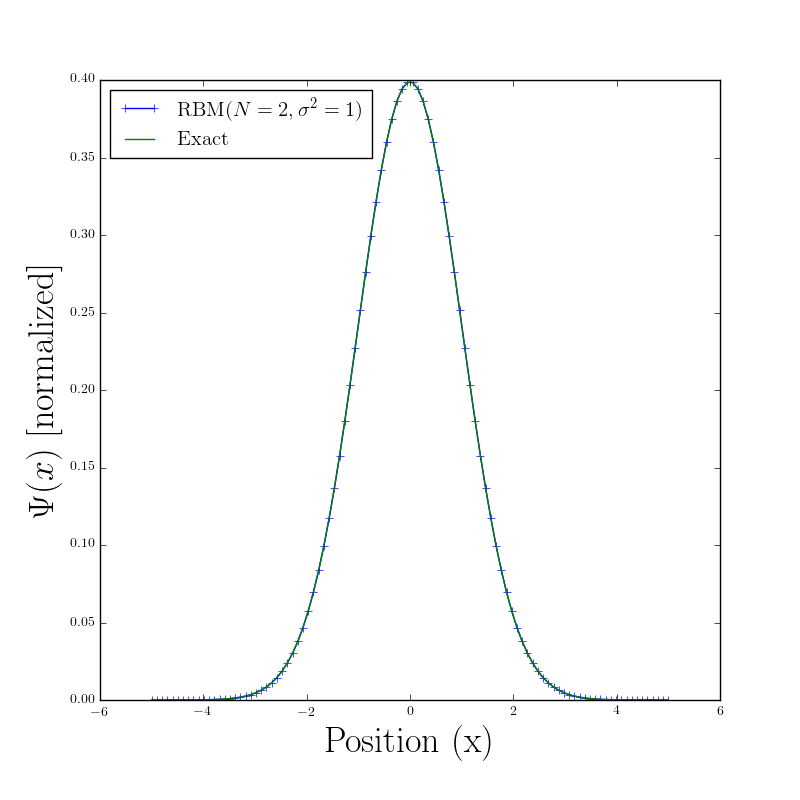
\includegraphics[width=0.8\linewidth]{../results/rbm-1d-1p.png}
    \caption{Ideal and learned wavefunction for one particle in one dimension.}
    \label{fig:rbm-1d-1p}
\end{figure}

\begin{multicols}{2}
    
    
    \autoref{fig:rbm-training-samplers} shows the error we make as a function of
    training iterations for the three different samplers discussed. We can
    observe a couple of interesting points from this plot. First, brute force
    Metropolis sampling has, as expected, a significantly higher variance in
    energy compared with Metropolis-Hastings. Interestingly that does not appear
    to affect the learning much, as both algorithms follow roughly the same
    curve. However, we would prefer to use Metropolis-Hastings here due to the
    stability it provides. 

    Gibbs sampling affects the training in a noticeably different way. We see it
    starting out with slower convergence compared the others, but as we continue
    to train, the Gibbs sampling curve holds a steeper decline, and surpassing
    the results obtained by the Metropolis variants. The effect is small though,
    keeping in mind the logarithmic y-axis which acts to amplify such
    differences. In fact, only the slightly slower start is always reproduced,
    as we sometimes get stuck in a local minimum before Gibbs can catch up
    fully.

    One thing to note is that the constant value assumed for $\sigma^2$ here was
    $\sigma^2=1$ for the Metropolis variants, and $\sigma^2=\flatfrac{1}{2}$ for
    Gibbs. Both of these were chosen so that setting $\vec\alpha=\vec 0$ would
    correspond to the ideal wavefunction. Using $\sigma^2=1$ with Gibbs makes it
    significantly worse. While this could potentially be helped by adding more
    parameters to the model (i.e. increasing $N$), this illustrates the
    potential issue with this general approach, namely the dependence on
    somewhat decent starting points.


\end{multicols}

\begin{figure}[ht]
    \centering
    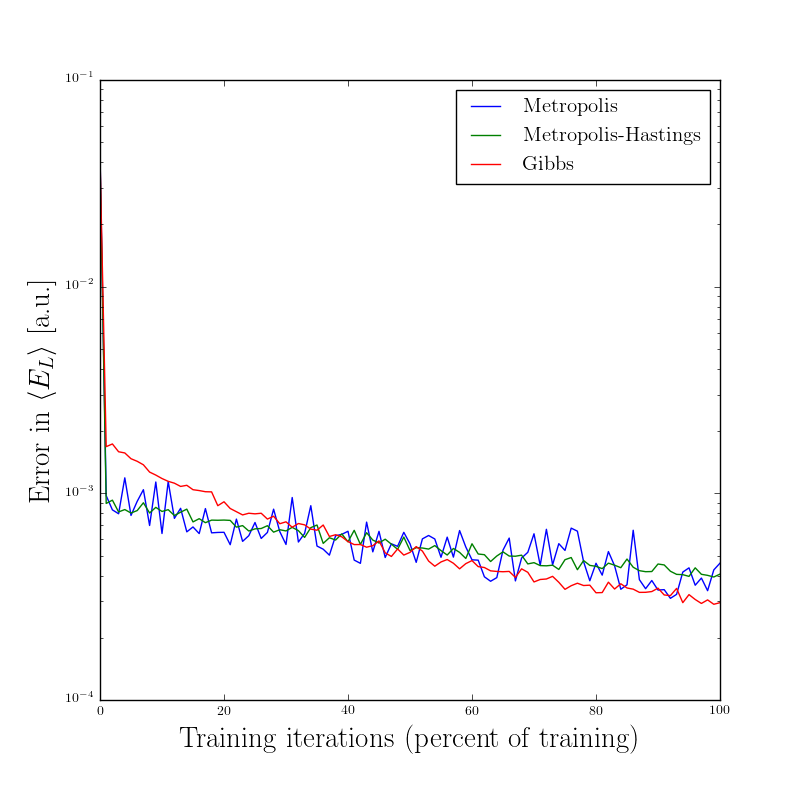
\includegraphics[width=0.8\linewidth]{../results/learning-samplers.png}
    \caption{Learning progression, comparing the three different sampling
    algorithms. We see a slight difference, especially in the jaggedness of the
    curve, indicating a difference in variance.}
    \label{fig:rbm-training-samplers}
\end{figure}


\begin{multicols}{2}

    \autoref{fig:rbm-training-optimizers} shows a similar comparison but for
    various optimizers. We can see that choosing a smaller learning rate for SGD
    results in slower convergence. Ideally, given sufficient training iterations
    we expect the smaller $\eta$ to result in slightly better accuracy, as it
    allows for more fine tuned adjustments. However, this is only guaranteed for
    ideally convex cost functions. Here we observe the small-$\eta$ optimizer
    getting stuck at some local minimum, unable to get out due to the small
    learning rate. This goes to show the importance of choosing a suitable
    learning rate when using vanilla SGD. Although not shown here, choosing to
    large values can result in catastrophic results.

    Better than both other methods is the Adam optmizer, here used with the
    default parameters given by the original authors~\cite{KingmaB14}. Although
    the large-$\eta$ SGD variant is initially somewhat faster, Adam ends up
    close to an order of magnitude better. Interestingly we appear to reach a
    point were further training reduces the energy slightly, while the variance
    remains roughly the same (causing an apparent increase in variance, due to
    the log-axis). In addition to the improved results, the main appeal of Adam
    is how well it performs without hyper-parameter tuning. Due to its adaptive
    nature, it performs well with the defaults in all scenarios attempted.
\end{multicols}

\begin{figure}[ht]
    \centering
    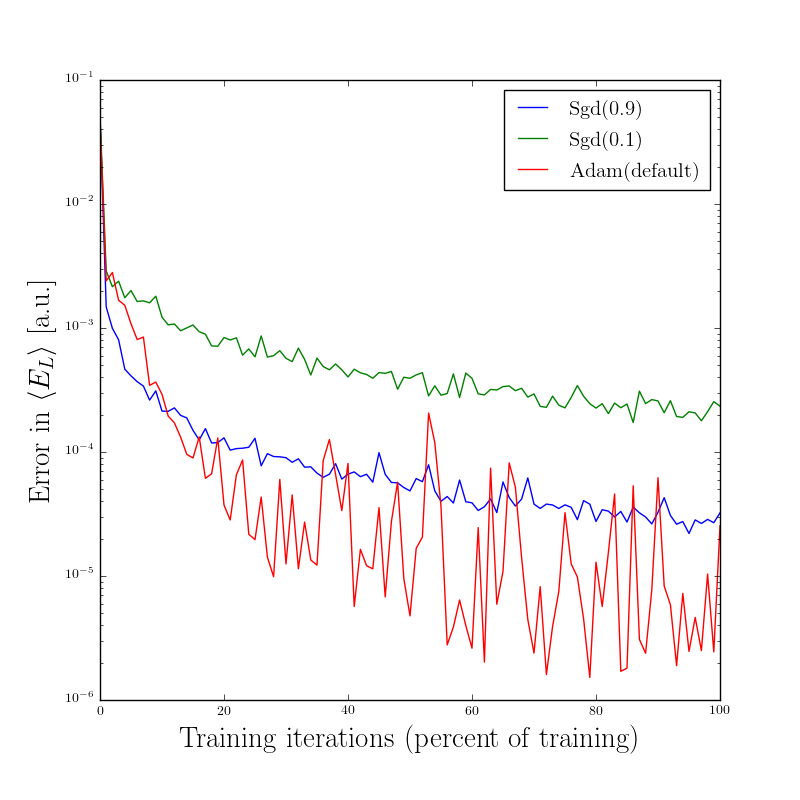
\includegraphics[width=0.8\linewidth]{../results/learning-optimizers.png}
    \caption{Learning progression, comparing different optimization algorithms.
    We observe Adam outperforming SGD, with the small learning rate converging
    very slowly. Training was performed using $\num{4e4}$ iterations with $100$
    samples per iterations.}
    \label{fig:rbm-training-optimizers}
\end{figure}


\begin{multicols}{2}

    \autoref{fig:rbm-training-N} shows yet again a similar plot of training
    progression, this time for various values for $N$. Here we see that
    increasing $N$ only served to slow down convergence significantly, as well
    as increasing the run-time. This results makes sense, considering that the
    ideal case has an optimum for $\vec \alpha=\vec 0$. Adding more parameters
    just means it gets harder for the optimizer to locate the minimum, and
    increases the density of local, non-optimal minima. Increasing $N$ might be
    more interesting when we consider the non-trivial interacting case.

    \printbibliography

\end{multicols}

\begin{figure}[ht]
    \centering
    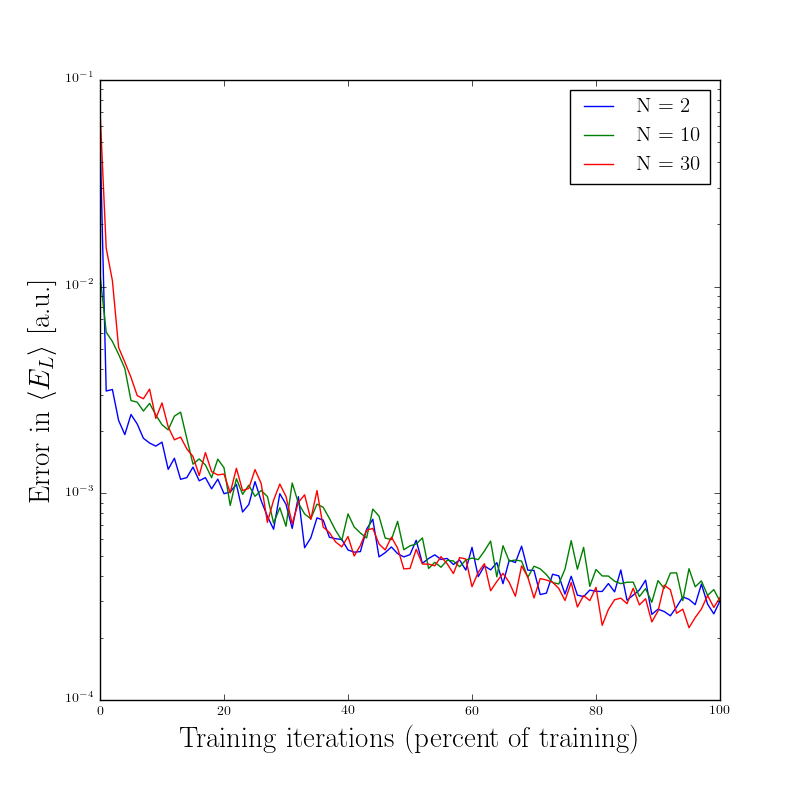
\includegraphics[width=0.8\linewidth]{../results/learning-N-variants.png}
    \caption{Learning progression, comparing different number of hidden neurons.
    Training was performed using $\num{4e4}$ iterations with $100$
    samples per iterations, using Metropolis-Hastings sampling and Adam
    optimizer.}
    \label{fig:rbm-training-N}
\end{figure}

\pagebreak
\begin{multicols}{2}
    \appendix
    \addcontentsline{toc}{section}{Appendices}
    \section*{Appendices}

    \section{Analytic Expression for the Local Energy}
    \label{app:E-L-derivation}
    
    To get started we will be needing a couple of partial derivatives:
   \begin{align}
        \pdv{}{X_k} (1+e^{v_j}) &=e^{v_j}\pdv{}{X_k}v_j =
        e^{v_j} \frac{w_{kj}}{\sigma^2}\\
        \begin{split}
        \pdv{}{X_k}e^{-\sum_i^M u_i} &= e^{-\sum_i^M
        u_i}\pdv{}{X_k}\qty(-\sum_i^M u_i) \\
        &= e^{-\sum_i^M u_i}\pdv{}{X_k} (-u_k) \\
        &= -e^{-\sum_i^M u_i} \frac{x_k-a_k}{\sigma^2}
        \end{split}
    \end{align}

    We are now ready to compute the first derivate:
    \begin{align*}
        \pdv{}{X_k}\Psi &= \frac{1}{Z} \left[\prod_j^N
        \qty(1+e^{v_j})\pdv{}{X_k}e^{-\sum_i^M u_i}\right.\\
        &\quad{  }\quad{    }\left. + e^{-\sum_i^M
        u_i}\pdv{}{X_k} \prod_j^N \qty(1+e^{v_j})\right]\\
        &= -\frac{x_k-a_k}{\sigma^2}\Psi + \Psi \sum_j^N
        \qty(\frac{1}{1+e^{v_j}}\pdv{}{X_k}\qty(1+e^{v_j}))\\
        &= -\frac{x_k-a_k}{\sigma^2}\Psi + \Psi\sum_j^N
        \frac{1}{1+e^{v_j}}\qty(\frac{w_{kj}}{\sigma^2} e^{v_j})\\
        &= \frac{1}{\sigma^2}\qty(a_k-x_k + \sum_j^N
        \frac{w_{kj}}{1+e^{-v_j}})\Psi.
    \end{align*}

    Before jumping into the second derivative, one more helpful derivative:
    \begin{align}
        \begin{split}
        \pdv{}{X_k}\qty(\frac{w_{kj}}{1+e^{-v_j}}) &=
            -w_{kj}\frac{e^{-v_j}}{\qty(1+e^{-v_j})^2}\pdv{(-v_j)}{X_k}\\
        &= \frac{w_{kj}^2}{\sigma^2} \frac{e^{-v_j}}{\qty(1+e^{-v_j})^2}
        \end{split}
    \end{align}

    Now, finally the second derivative:
    \begin{align*}
        \frac{1}{\Psi}\pdv[2]{}{X_k}\Psi &= \frac{1}{\Psi}\pdv{}{X_k}\qty[\frac{1}{\sigma^2}\qty(a_k-x_k + \sum_j^N
        \frac{w_{kj}}{1+e^{-v_j}})\Psi]\\
        &= \frac{1}{\sigma^2} \left[ \pdv{}{X_k}\qty(a_k-x_k + \sum_j^N
        \frac{w_{kj}}{1+e^{-v_j}} )   \right.\\
        &\quad{   }\quad{   } \left. 
        + \qty(a_k-x_k + \sum_j^N
        \frac{w_{kj}}{1+e^{-v_j}})\frac{1}{\Psi}\pdv{}{X_k}\Psi 
        \right]\\
        \begin{split}
        &= -\frac{1}{\sigma^2} + \sum_j^N
        \frac{w_{kj}^2}{\sigma^4}
        \frac{e^{-v_j}}{\qty(1+e^{-v_j})^2} \\
        &\quad{   }\quad{      }  +
        \frac{1}{\sigma^4}\qty(a_k-x_k+\sum_j^N \frac{w_{kj}}{1+e^{-v_j}})^2
        \end{split}\numberthis\label{eq:E-L-second-deriv}
    \end{align*}


    The final expression we shall use then for the local energy is:

    \begin{align}
        E_L &= \sum_{i=1}^P \frac{1}{2}r_i^2 + \sum_{i<j}^{P} \frac{1}{r_{ij}}
        - \frac{1}{2} \sum_{k=1}^M
        \frac{1}{\Psi}\pdv[2]{}{x_k}\Psi,\label{eq:E-L-final}
    \end{align}
    substituting in \autoref{eq:E-L-second-deriv}.

\end{multicols}



\end{document}
